\newpage
\section{HIMA Software (ELOP II-NT)}
The second part of the lab was used to become more familiar with the ELOP II-NT software and design a simple program, which gave a quick glimpse of the powerful software.

\subsection{Tutorial and modules}
Configuring the system was easy thanks to the guide provided, where the logic entry was preformed by simple Drag & Drop from the standard libraries. 

The input module was recognized to be  F3236  rack 2 position 1 and 2.
Output module F3330 rack 2, position 4 and 5.

\begin{figure}[!htb]
    \centering
    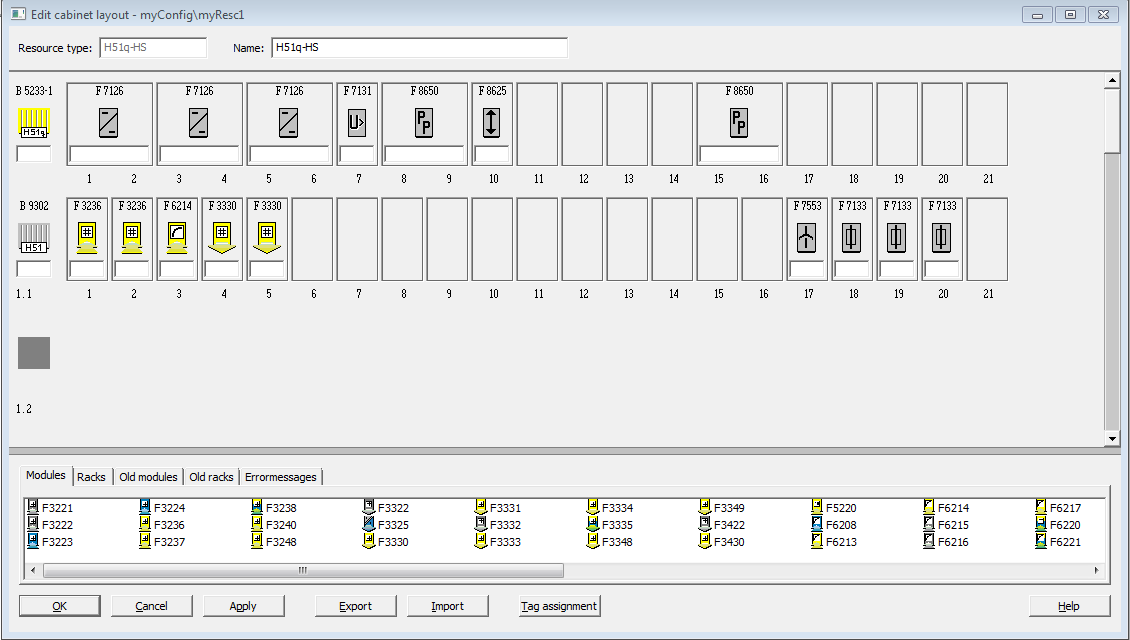
\includegraphics[scale=0.55]{images/2b1}
     \caption{Cabinet Layout}
\end{figure}

The test program was to create a simple AND logic which turned on the LED when both inputs where ON, and OFF when one of them was low.



\subsection{What is BUSCOM}
The serial communication between HIMA PES and external systems is called BUSCOM, it is used for configuration and programming.


\subsection{2oo3 analog votering}
The 2oo3 analog votering was created by creating multiple sub-blocks and connecting them together to achieve the wanted result. The Figure below shows the final result, this logic was tested in both offline mode, using OLT fields and online mode using the outout module to turn the light diodes on/off.
\begin{figure}[!htb]
    \centering
    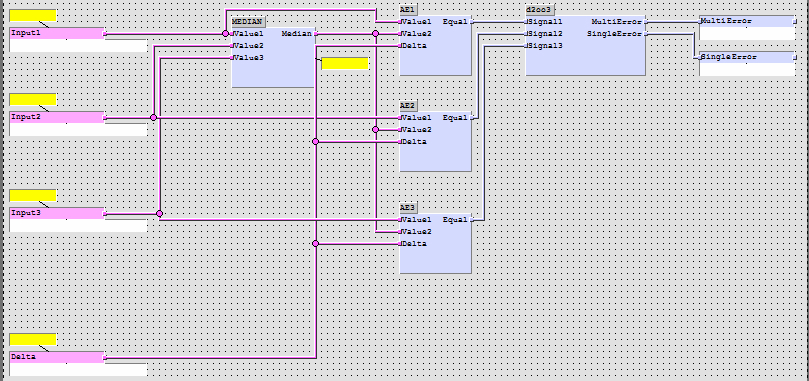
\includegraphics[scale=0.55]{images/A2oo3}
     \caption{2oo3 Analog Votering}
\end{figure}

\begin{figure}[!htb]
    \centering
    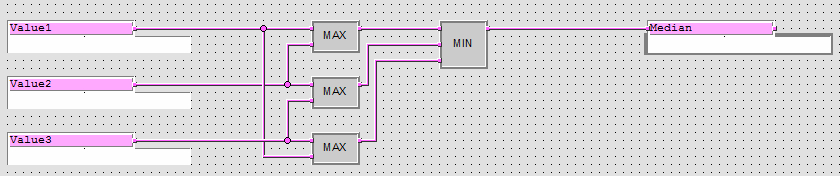
\includegraphics[scale=0.4]{images/Median}
     \caption{Median Block}
\end{figure}

\begin{figure}[!htb]
    \centering
    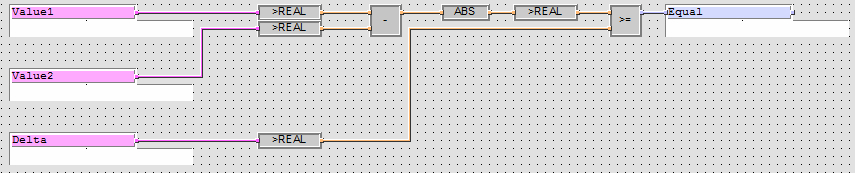
\includegraphics[scale=0.45]{images/AE}
     \caption{Almost Equal Block}
\end{figure}

\begin{figure}[!htb]
    \centering
    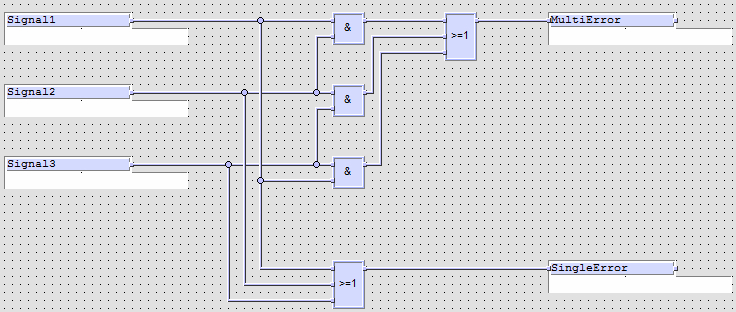
\includegraphics[scale=0.45]{images/d2oo3}
     \caption{d2oo3 Block}
\end{figure}

\subsection{HA-RTE-3 and a2oo3}
In the last part, the already created logic was combined with the HA-RTE-3 module, the figure below shows the connection between the modules.
\begin{figure}[!htb]
    \centering
    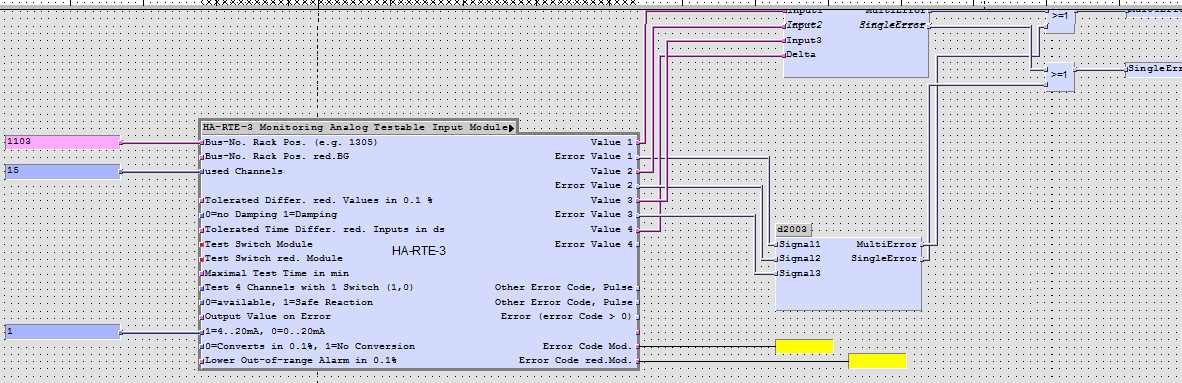
\includegraphics[scale=0.4]{images/del2f}
     \caption{HA-RTE-3 }
\end{figure}